
\chapter{Statistics and Probability}
\section{Definition of Moments}
Let $x\in\mathbb R^{n}$ is a random variable.
We write $m = E[x]\in\mathbb R^n$ for the expectation and
$M=\mathrm{Var}[x] = E[(x-m)(x-m)^T]$ for the covariance (when these quantities are defined.)

In tensor diagrams, we will use square brackets:
\[
   \vecmatvec{1em}{}{}{m}
   =
\mathbin{\begin{tikzpicture}[baseline=(n0.base), inner sep=1pt]
   \node (n0) at (0,0) {$[$};
   \node [right=1em of n0] (n1) {$x]$};
   \draw (n0) -- (n1);
\end{tikzpicture}}
\quad\text{and}\quad
   \vecmatvec{1em}{}{M}{}
   =
\mathbin{\begin{tikzpicture}[baseline=(n0.base), inner sep=1pt]
   \node (n0) at (0,0) {$[$};
   \node [right=1em of n0] (n1) {$(x\ominus m)$};
   \node [right=.5em of n1] (n2) {$(x\ominus m)$};
   \node [right=1em of n2] (n3) {$]$};
   \draw (n0) -- (n1);
   \draw (n2) -- (n3);
\end{tikzpicture}}
\]
We will use the circled minus, $\ominus$, to distinguish the operation from contraction edges.

We can also define the third and fourth centralized moment tensors
\[
   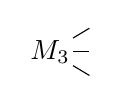
\begin{tikzpicture}[baseline=(T.base), inner sep=1pt]
      \node (T) {$M_3$};
      \draw (T) -- ++(.5,.3);
      \draw (T) -- ++(.5,-.3);
      \draw (T) -- ++(.5,0);
   \end{tikzpicture}
   =
   \renewcommand*{\arraystretch}{1.3}
   \begin{bmatrix}
      \vecmatvec{1em}{(x\ominus m)}{}{} \\
      \vecmatvec{1em}{(x\ominus m)}{}{} \\
      \vecmatvec{1em}{(x\ominus m)}{}{}
   \end{bmatrix}
\quad\text{and}\quad
   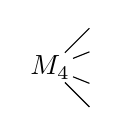
\begin{tikzpicture}[baseline=(T.base), inner sep=1pt]
      \node (T) {$M_4$};
      \draw (T) -- ++(.5,.5);
      \draw (T) -- ++(.5,-.5);
      \draw (T) -- ++(.5,.2);
      \draw (T) -- ++(.5,-.2);
   \end{tikzpicture}
   =
   \renewcommand*{\arraystretch}{1.3}
   \begin{bmatrix}
      \vecmatvec{1em}{(x\ominus m)}{}{} \\
      \vecmatvec{1em}{(x\ominus m)}{}{} \\
      \vecmatvec{1em}{(x\ominus m)}{}{} \\
      \vecmatvec{1em}{(x\ominus m)}{}{}
   \end{bmatrix}
.
\]
%These are less common in introductory causes, even though the scalar third and fourth moment are common.
%This is presumably because they require higher order tensors.

%If the entries of $x$ are independent, the non-diagonal entries disappear, so we get
%\[
%M =
%\left[
%   \begin{tikzpicture}[baseline=(c.base), inner sep=1pt]
%      \node (T1) {$(x\ominus m)$};
%      \node (T2)[below=.5em of T1] {$(x\ominus m)$};
%      \node (c)[right=.7em of T1, yshift=-1em] {$\sbullet$};
%      \draw (T1) -- (c);
%      \draw (T2) -- (c);
%      \draw (c) -- ++(.7em,0);
%   \end{tikzpicture}
%\right]
%\quad\text{and}\quad
%M_3 =
%\left[
%   \begin{tikzpicture}[baseline=(T2.base), inner sep=1pt]
%      \node (T1) {$(x\ominus m)$};
%      \node (T2)[below=.5em of T1] {$(x\ominus m)$};
%      \node (T3)[below=.5em of T2] {$(x\ominus m)$};
%      \node (c)[right=.7em of T2] {$\sbullet$};
%      \draw (T1) -- (c);
%      \draw (T2) -- (c);
%      \draw (T3) -- (c);
%      \draw (c) -- ++(.7em,0);
%   \end{tikzpicture}
%\right]
%\quad\text{and so on.}
%\]
% If the entries are also identically distributed, we simply have
% \[
%    M = \sigma^2
%    \,
% \begin{tikzpicture}[baseline=(T.base), inner sep=0]
%    \node (T) {$\sbullet$};
%    \draw (T) -- ++(0,.3);
%    \draw (T) -- ++(0,-.3);
% \end{tikzpicture}
%    \text{ and }
%    M_3 = \mathrm{E}[(x_0-m_0)^3]
% \begin{tikzpicture}[baseline=(T.base), inner sep=0]
%    \node (T) {$\sbullet$};
%    \draw (T) -- ++(0,.3);
%    \draw (T) -- ++(-.2,-.3);
%    \draw (T) -- ++(.2,-.3);
% \end{tikzpicture}
% .
% \]


\subsection{Expectation of Linear Combinations}
General principle: The ``linearity of expectation'' lets you pull out all parts of the graph not involving $X$.
\[
   \vcenter{\hbox{
      \import{figures/}{linearityOfExpectation.pdf_tex}
   }}
\]
where $M_3$ is the expectation\footnote{FIXME: This is different from the notation just introduced above.}
\(
\left[
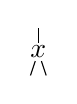
\begin{tikzpicture}[baseline=(T.base), inner sep=1pt]
   \node (T) {$x$};
   \draw (T) -- ++(0,.3);
   \draw (T) -- ++(-.1,-.3);
   \draw (T) -- ++(.1,-.3);
\end{tikzpicture}
\,
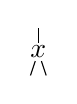
\begin{tikzpicture}[baseline=(T.base), inner sep=1pt]
   \node (T) {$x$};
   \draw (T) -- ++(0,.3);
   \draw (T) -- ++(-.1,-.3);
   \draw (T) -- ++(.1,-.3);
\end{tikzpicture}
\,
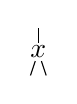
\begin{tikzpicture}[baseline=(T.base), inner sep=1pt]
   \node (T) {$x$};
   \draw (T) -- ++(0,.3);
   \draw (T) -- ++(-.1,-.3);
   \draw (T) -- ++(.1,-.3);
\end{tikzpicture}
\right]
\),
which is an order-9 tensor with no dependence on the constants $A$, $B$, $C$ and $D$.
In practice you would want to name the edges to keep track of what gets multiplied with what.

We can even use linearity of expectation to push the expectation inside an infinite sum of tensors, as in the following moment generating function, which relates all the $M_k$ tensors:
\begin{align*}
   \mathrm{E}(\mathrm{e}^{\langle x\ominus m, t\rangle})
   &= \sum_{k=0}^\infty \frac{1}{k!} \mathrm{E}[\langle x\ominus m, t\rangle^k]
    = \mathrm{E}\big[\sum_{k=0}^\infty \frac{1}{k!} \langle (x\ominus m)^{\otimes k}, t^{\otimes k}\rangle\big]
   = \sum_{k=0}^\infty \frac{1}{k!} \langle M_k, t^{\otimes k}\rangle
 \\&=
  % =
   1
   +
   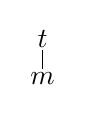
\begin{tikzpicture}[baseline=.5em, inner sep=1]
      \node (T) {$m$};
      \draw (T) -- ++(0,.5) node[fill=white] {$t$};
   \end{tikzpicture}
   +
   \frac{1}{2}
   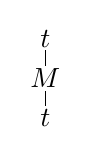
\begin{tikzpicture}[baseline=(T.base), inner sep=1]
      \node (T) {$M$};
      \draw (T) -- ++(0,.5) node[fill=white] {$t$};
      \draw (T) -- ++(0,-.5) node[fill=white] {$t$};
   \end{tikzpicture}
   +
   \frac{1}{6}
   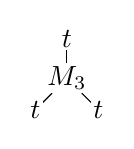
\begin{tikzpicture}[baseline=(T.base), inner sep=1]
      \node (T) {$M_3$};
      \draw (T) -- ++(0,.5) node[fill=white] {$t$};
      \draw (T) -- ++(-.4,-.4) node[fill=white] {$t$};
      \draw (T) -- ++(.4,-.4) node[fill=white] {$t$};
   \end{tikzpicture}
   +
   \frac{1}{24}
   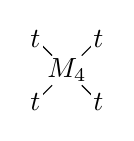
\begin{tikzpicture}[baseline=(T.base), inner sep=1]
      \node (T) {$M_4$};
      \draw (T) -- ++(-.4,-.4) node[fill=white] {$t$};
      \draw (T) -- ++(.4,-.4) node[fill=white] {$t$};
      \draw (T) -- ++(-.4,.4) node[fill=white] {$t$};
      \draw (T) -- ++(.4,.4) node[fill=white] {$t$};
   \end{tikzpicture}
   +
   \dots
\end{align*}

\subsection{Linear Forms}
The Matrix Cookbook gives the following simple expectation:
\begin{walign}
   \tag{312}
   \E[AXB+C] &= A \E[X] B + C
   &
   \renewcommand*{\arraystretch}{1.3}
   \begin{bmatrix}
      \matmul{A,X,B} \\+\, \matmul{C}
   \end{bmatrix}
   &=
   \renewcommand*{\arraystretch}{1.3}
   \begin{matrix}
      \matmul{A,[X],B} \\+\, \matmul{C}
   \end{matrix}
\end{walign}

\subsection{Quadratic Forms}
We often prefer to write expectations in terms of the simple centered moments, which we can do by pulling out the mean:
\renewcommand*{\arraystretch}{1}
\[
   \begin{bmatrix}
      x - \\
      x -
   \end{bmatrix}
   =
   \begin{bmatrix}
      (x\ominus m) - \\
      (x\ominus m) -
   \end{bmatrix}
   +
   \begin{array}{c}
      m - \\
      m -
   \end{array}
   =
   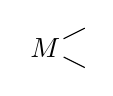
\begin{tikzpicture}[baseline=(T.base), inner sep=1pt]
      \node (T) {$M$};
      \draw (T) -- ++(.5,.25);
      \draw (T) -- ++(.5,-.25);
   \end{tikzpicture}
   +
   \begin{array}{c}
      m - \\
      m -
   \end{array}
\]
This makes it easy to handle the quadratic forms from the Matrix Cookbook:
\begin{walign}
   \tag{313}
   \mathrm{Var}[Ax] &= A \mathrm{Var}[x] A^T
   &
   \renewcommand*{\arraystretch}{1.3}
   \begin{bmatrix}
      \vecmatvec{.5em}{A}{}{x} \ominus [\vecmatvec{.5em}{A}{}{x}] \\
      \vecmatvec{.5em}{A}{}{x} \ominus [\vecmatvec{.5em}{A}{}{x}]
   \end{bmatrix}
   &=
   \renewcommand*{\arraystretch}{1.3}
   \begin{bmatrix}
      \vecmatvec{.5em}{A}{}{(x\ominus m)} \\
      \vecmatvec{.5em}{A}{}{(x\ominus m)}
   \end{bmatrix}
 \\&&&=
   \vcenter{\hbox{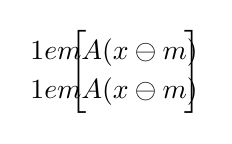
\begin{tikzpicture}[inner sep=1pt]
      \node (n1) at (0,-.25) {$\vecmatvec{1em}{A}{}{(x\ominus m)}$};
      \node (n2) at (0,.25) {$\vecmatvec{1em}{A}{}{(x\ominus m)}$};
      \node at (-.45, 0) {$\Bigg[$};
      \node at (1, 0) {$\Bigg]$};
   \end{tikzpicture}}}
 \\&&& =
   \vecmatvec{.5em}{}{A,M_2,A}{}
%%%%%%%%%%%%%%%%%%%%%%%%%%%%%%%%%%%%%%%%%%%%%%%%%%%%%%%%%%%%%%%%%%%%%%%%%%%%%%%%
   \\[.5em]
   \tag{318}
   \E[x^T A x]
   &= \mathrm{Tr}(A M) + m^T A m
   &
   [\vecmatvec{.5em}{x}{A}{x}]
   &=
   \left(
      \begin{bmatrix}
         (x\ominus m) - \\
         (x\ominus m) -
      \end{bmatrix}
      +
      \begin{array}{c}
         m - \\
         m -
      \end{array}
   \right)
   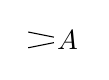
\begin{tikzpicture}[baseline=(A.base), inner sep=1pt]
      \node (A) {$A$};
      \draw (A) -- ++(-.5, .1);
      \draw (A) -- ++(-.5, -.1);
   \end{tikzpicture}
   \\
   &&&=
   \mathbin{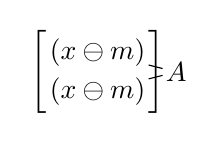
\begin{tikzpicture}[baseline=(A.base), inner sep=1pt]
      \node (n1) at (0,-.25) {$(x\ominus m)$};
      \node (n2) at (0,.25) {$(x\ominus m)$};
      \node at (-.75, 0) {$\Bigg[$};
      \node at (.75, 0) {$\Bigg]$};
      \node (A) at (1, 0) {$A$};
      \draw (n1) -- (A);
      \draw (n2) -- (A);
   \end{tikzpicture}}
   +
   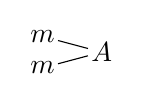
\begin{tikzpicture}[baseline=(A.base), inner sep=1pt]
      \node (A) {$A$};
      \node (m1) at (-.75, .2) {$m$};
      \node (m2) at (-.75, -.2) {$m$};
      \draw (m1) -- (A) -- (m2);
   \end{tikzpicture}
   \\
   &&&=
   \trace{M,A}2
   +
   \vecmatvec{.5em}{m}{A}{m}
   \\[.5em]
\end{walign}

\begin{align*}
   E[(A\mathbf{x} + a)(B\mathbf{x} + b)^T] &= AMB^T + (Am + a)(Bm + b)^T \tag{320} \\
   E[\mathbf{x}\mathbf{x}^T] &= M + mm^T \tag{321} \\
   E[\mathbf{x} a^T \mathbf{x}] &= (M + mm^T)a \tag{322} \\
   E[\mathbf{x}^T a\mathbf{x}^T] &= a^T(M + mm^T) \tag{323} \\
   E[(A\mathbf{x})(A\mathbf{x})^T] &= A(M + mm^T)A^T \tag{324} \\
   E[(\mathbf{x} + a)(\mathbf{x} + a)^T] &= M + (m + a)(m + a)^T \tag{325} \\
   E[(A\mathbf{x} + a)^T(B\mathbf{x} + b)] &= \text{Tr}(AMB^T) + (Am + a)^T(Bm + b) \tag{326} \\
   E[\mathbf{x}^T \mathbf{x}] &= \text{Tr}(M) + m^T m \tag{327} \\
   E[\mathbf{x}^T A\mathbf{x}] &= \text{Tr}(AM) + m^T Am \tag{328} \\
   E[(A\mathbf{x})^T(A\mathbf{x})] &= \text{Tr}(AMA^T) + (Am)^T(Am) \tag{329} \\
   E[(\mathbf{x} + a)^T(\mathbf{x} + a)] &= \text{Tr}(M) + (m + a)^T(m + a) \tag{330}
\end{align*}



\subsection{Cubic Forms}

\[
\begin{tikzpicture}[scale=1.3,
  every node/.style={inner sep=1pt, circle, draw, fill=white, thin},
  label/.style={draw=none, fill=none, text=black, font=\scriptsize},
  declare function={
    xgap=.8;  % Horizontal spacing between diagrams
  }]

  \drawPartitionAtAngle{(-1.6*xgap,0)}{3}{$\kappa_3$}{{{1,2,3}}}
  \drawPartitionAtAngle{(0,0)}{3}{$+\kappa_2\kappa_1\Big($}{{{1,2},{3}}}
  \drawPartitionAtAngle{(xgap,0)}{3}{$+$}{{{1,3},{2}}}
  \drawPartitionAtAngle{(2*xgap,0)}{3}{$+$}{{{2,3},{1}}}
  \drawPartitionAtAngle{(3.6*xgap,0)}{3}{$\Big)+\kappa_1^3$}{{{1},{2},{3}}}

\end{tikzpicture}
\]


When $x$ is a stochastic vector with mean vector $m$,
it can be convenient to expand the raw third moment in terms of the central moments:

\renewcommand*{\arraystretch}{1}
\begin{align*}
\begin{bmatrix}
   x - \\
   x - \\
   x -
\end{bmatrix}
&=
\begin{bmatrix}
   (x\ominus m) - \\
   (x\ominus m) - \\
   (x\ominus m) -
\end{bmatrix}
\vspace{-.5em}
+
3
\hspace{-.25em}
\begin{array}{l}
\begin{bmatrix}
   (x\ominus m) -
\end{bmatrix}\\[.1em]
\begin{bmatrix}
   m - \\
   m -
\end{bmatrix}
\end{array}
\hspace{-.5em}
+
3
\hspace{-.25em}
\begin{array}{l}
\begin{bmatrix}
   m -
\end{bmatrix}\\[.1em]
\begin{bmatrix}
   (x\ominus m) - \\
   (x\ominus m) -
\end{bmatrix}
\end{array}
\hspace{-.5em}
+
\hspace{-.5em}
\begin{array}{c}
\begin{bmatrix}
   m -
\end{bmatrix}\\[.1em]
\begin{bmatrix}
   m -
\end{bmatrix}\\[.1em]
\begin{bmatrix}
   m -
\end{bmatrix}
\end{array}
%
\\&=
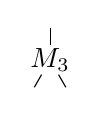
\begin{tikzpicture}[baseline=(T.base), inner sep=1pt]
   \node (T) {$M_3$};
   \draw (T) -- ++(0,.4);
   \draw (T) -- ++(-.2,-.35);
   \draw (T) -- ++(.2,-.35);
\end{tikzpicture}
+
3
\hspace{-.25em}
\begin{array}{c}
   m - \\
   -M-
\end{array}
\hspace{-.5em}
+
\begin{array}{c}
   m - \\
   m - \\
   m -
\end{array}
\end{align*}
TODO: The edges from the $m,M$ term needs to be symmetrized.


But this is still a bit of a mess.
See also below on Cumulants.



Assume \(\mathbf{x}\) to be a stochastic vector with independent coordinates, mean \(m\),
covariance \(M\) and central moments \(v_3 = \mathbb{E}[(\mathbf{x} - m)^3]\). Then (see [7])
\begin{align*}
&\mathbb{E}[(A\mathbf{x} + a)(B\mathbf{x} + b)^T (C\mathbf{x} + c)]
\\&\quad=
A\,\mathrm{diag}(B^T C) v_3
\\&\quad+
(Am + a) \mathrm{Tr}(BMC^T)
\\&\quad+
AMC^T (Bm + b)
\\&\quad\,+
AMB^T (Cm + c)
\\&\quad+
(Am + a)(Bm + b)^T (Cm + c)
\\
  &\mathbb{E}[\mathbf{x} \mathbf{x}^T \mathbf{x}]
\\&\quad=
   v_3
\\&\quad+
   2 Mm
\\&\quad+
   (\text{Tr}(M) + m^T m) m
\end{align*}


\section{Cumulants}

Given a random vector $x\in\mathbb R^d$,
its $n$th Cumulant Tensor, $K_n\in\R^{d,\ldots,d}$ is defined by
\[
   \log \mathrm{E}(\mathrm{e}^{\langle t, x\rangle})
   = \sum_{n=1}^\infty \frac{1}{n!} \langle K_n, t^{\otimes n}\rangle
   =
   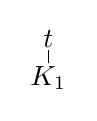
\begin{tikzpicture}[baseline=.5em, inner sep=1]
      \node (T) {$K_1$};
      \draw (T) -- ++(0,.5) node[fill=white] {$t$};
   \end{tikzpicture}
   +
   \frac{1}{2}
   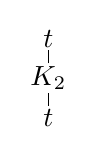
\begin{tikzpicture}[baseline=(T.base), inner sep=1]
      \node (T) {$K_2$};
      \draw (T) -- ++(0,.5) node[fill=white] {$t$};
      \draw (T) -- ++(0,-.5) node[fill=white] {$t$};
   \end{tikzpicture}
   +
   \frac{1}{6}
   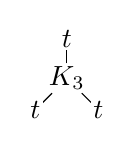
\begin{tikzpicture}[baseline=(T.base), inner sep=1]
      \node (T) {$K_3$};
      \draw (T) -- ++(0,.5) node[fill=white] {$t$};
      \draw (T) -- ++(-.4,-.4) node[fill=white] {$t$};
      \draw (T) -- ++(.4,-.4) node[fill=white] {$t$};
   \end{tikzpicture}
   +
   \dots
\]
The first couple of cumulants are similar to the central moments:
\[
   K_1 = m
   \quad\text{and}\quad
   K_2 = M
   \quad\text{and}\quad
   K_3 = M_3
   \quad\text{and}\quad
   K_4 = M_4
   - \begin{tikzpicture}[baseline=-.8em, inner sep=.5pt]
      \node (M1) {\scriptsize $M_2$};
      \node[below=.4em of M1] (M2) {\scriptsize $M_2$};
      \draw (M1) -- ++(.35,0);
      \draw (M2) -- ++(.35,0);
      \draw (M1) -- ++(-.35,0);
      \draw (M2) -- ++(-.35,0);
   \end{tikzpicture}
   - \begin{tikzpicture}[baseline=(M1.base), inner sep=.5pt]
      \node (M1) {\scriptsize $M_2$};
      \node[right=.05em of M1] (M2) {\scriptsize $M_2$};
      \draw (M1) -- ++(-.25,.25);
      \draw (M1) -- ++(-.25,-.25);
      \draw (M2) -- ++(.25,.25);
      \draw (M2) -- ++(.25,-.25);
   \end{tikzpicture}
   - \begin{tikzpicture}[baseline=(M1.base), inner sep=.5pt]
      \node (M1) {\scriptsize $M_2$};
      \node[right=.05em of M1, yshift=-2pt] (M2) {\scriptsize $M_2$};
      \draw (M1) -- ++(-.25,.25);
      \draw (M1) -- ++(+.7,-.25);
      \draw (M2) -- ++(-.7,-.25);
      \draw (M2) -- ++(.25,.25);
   \end{tikzpicture}
   .
\]
They have the nice property (which is easy to see from the definition) that they are additive for independent random variables:
$
   K_n(x + y) = K_n(x) + K_n(y).
$
This generalizes the standard property that the variance of the sum of independent random variables is the sum of the variances.

We can write the expectations of $x^{\otimes n}$ in terms of the cumulants:

\[
   \begin{bmatrix}
      \begin{tikzpicture}[
         baseline=(T.base),
         every node/.style={inner sep=1pt, circle, draw=none, fill=white},
       ]
       \draw (30:.2) node[label] {$x$} -- (30:.6);
       \draw (150:.2) node[label] {$x$} -- (150:.6);
       \draw (270:.2) node[label] {$x$} -- (270:.6);
      \end{tikzpicture}
   \end{bmatrix}
   =
   \begin{tikzpicture}[
      baseline=-1em,
     every node/.style={inner sep=1pt, circle, draw, fill=white, thin},
     label/.style={draw=none, fill=none, text=black, font=\scriptsize},
     declare function={
       xgap=1.8;  % Horizontal spacing between diagrams
     }]
     \drawPartitionAtAngle[k]{(-1*xgap,0)}{3}{}{{{1,2,3}}}
     \drawPartitionAtAngle[k]{(0,0)}{3}{$+$}{{{1,2},{3}}}
     \drawPartitionAtAngle[k]{(xgap,0)}{3}{$+$}{{{1,3},{2}}}
     \drawPartitionAtAngle[k]{(xgap*2,0)}{3}{$+$}{{{1},{2,3}}}
     \drawPartitionAtAngle[k]{(xgap*3,0)}{3}{$+$}{{{1},{2},{3}}}
   \end{tikzpicture}
   .
\]
In general the sum is over all the partitions of the set $\{1,\ldots,n\}$.

If the entries of $x$ are \emph{independent}, the off-diagonals of the cumulant tensors $K_1, K_2, \dots$ are zero.
This means 
%
Assume each $x_i$ has cumulants $\kappa_1, \kappa_2, \kappa_3, \kappa_4 \in \R$, then
\[
\begin{bmatrix}
   \begin{tikzpicture}[
      baseline=(T.base),
      every node/.style={inner sep=1pt, circle, draw=none, fill=white},
    ]
    \draw (30:.2) node[label] {$x$} -- (30:.5);
    \draw (120:.2) node[label] {$x$} -- (120:.5);
    \draw (210:.2) node[label] {$x$} -- (210:.5);
    \draw (300:.2) node[label] {$x$} -- (300:.5);
   \end{tikzpicture}
\end{bmatrix}
=
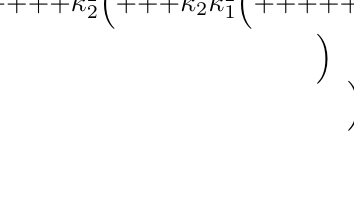
\begin{tikzpicture}[
  every node/.style={inner sep=1pt, circle, draw, fill=white, thin},
  label/.style={draw=none, fill=none, text=black, font=\scriptsize},
  declare function={
    xgap=1;  % Horizontal spacing between diagrams
    ygap=.6;  % Vertical spacing between rows
  },
  baseline=-1cm
  ]
  \pgfmathsetmacro{\outerRadius}{.3}
  \pgfmathsetmacro{\innerRadius}{.1}

  % Pattern {4} - 1 partition
  \drawPartitionAtAngle{(0,0)}{4}{$\kappa_4$}{{{1,2,3,4}}}

  % Pattern {3,1} - 4 partitions
  \drawPartitionAtAngle{(0,-ygap)}{4}{$+\kappa_3\kappa_1\Big($}{{{1,2,3},{4}}}
  \drawPartitionAtAngle{(xgap,-ygap)}{4}{$+$}{{{1,2,4},{3}}}
  \drawPartitionAtAngle{(2*xgap,-ygap)}{4}{$+$}{{{2},{1,3,4}}}
  \drawPartitionAtAngle{(3*xgap,-ygap)}{4}{$+$}{{{1},{2,3,4}}}
  \node[label] at (3.5*xgap,-ygap) {$\Big)$};

  % Pattern {2,2} - 3 partitions
  \drawPartitionAtAngle{(0,-2*ygap)}{4}{$+\kappa_2^2\Big($}{{{1,2},{3,4}}}
  \drawPartitionAtAngle{(xgap,-2*ygap)}{4}{$+$}{{{1,3},{2,4}}}
  \drawPartitionAtAngle{(2*xgap,-2*ygap)}{4}{$+$}{{{1,4},{2,3}}}
  \node[label] at (2.5*xgap,-2*ygap) {$\Big)$};

  % Pattern {2,1,1} - 6 partitions
  \drawPartitionAtAngle{(0,-3*ygap)}{4}{$+\kappa_2\kappa_1^2\Big($}{{{1,2},{3},{4}}}
  \drawPartitionAtAngle{(xgap,-3*ygap)}{4}{$+$}{{{1,3},{2},{4}}}
  \drawPartitionAtAngle{(2*xgap,-3*ygap)}{4}{$+$}{{{1,4},{2},{3}}}
  \drawPartitionAtAngle{(3*xgap,-3*ygap)}{4}{$+$}{{{1},{2,3},{4}}}
  \drawPartitionAtAngle{(4*xgap,-3*ygap)}{4}{$+$}{{{1},{3},{2,4}}}
  \drawPartitionAtAngle{(5*xgap,-3*ygap)}{4}{$+$}{{{1},{2},{3,4}}}
  \node[label] at (5.5*xgap,-3*ygap) {$\Big)$};

  % Pattern {1,1,1,1} - 1 partition
  \drawPartitionAtAngle{(0,-4*ygap)}{4}{$+\kappa_1^4$}{{{1},{2},{3},{4}}}

\end{tikzpicture}
\]

Note in particular, that if the mean, $\kappa_1$, is zero, only four terms survive.
%\(
%\begin{tikzpicture}[
%   baseline=4em,
%  every node/.style={inner sep=1pt, circle, draw, fill=white, thin},
%  label/.style={draw=none, fill=none, text=black, font=\scriptsize},
%  declare function={
%    xgap=1;  % Horizontal spacing between diagrams
%    ygap=.6;  % Vertical spacing between rows
%  },
%  baseline=-1cm
%  ]
%  \pgfmathsetmacro{\outerRadius}{.3}
%  \pgfmathsetmacro{\innerRadius}{.1}
%
%  \drawPartitionAtAngle{(-1.5*xgap,0)}{4}{$\kappa_4$}{{{1,2,3,4}}}
%  \drawPartitionAtAngle{(0,0)}{4}{$+\kappa_2^2\Big($}{{{1,2},{3,4}}}
%  \drawPartitionAtAngle{(xgap,0)}{4}{$+$}{{{1,3},{2,4}}}
%  \drawPartitionAtAngle{(2*xgap,0)}{4}{$+$}{{{1,4},{2,3}}}
%  \node[label] at (2.5*xgap,0) {$\Big)$};
%\end{tikzpicture}
%.
%\)
For $n=5$ there are 52 partitions in total, but only 11 survive if $\kappa_1=0$:
\[
   \begin{tikzpicture}[
     every node/.style={inner sep=1pt, circle, draw, fill=white, thin},
     label/.style={draw=none, fill=none, text=black, font=\scriptsize},
     declare function={
       xgap=1;  % Horizontal spacing between diagrams
       ygap=.6;  % Vertical spacing between rows
     },
     baseline=-1cm
     ]
     \pgfmathsetmacro{\outerRadius}{.3}
     \pgfmathsetmacro{\innerRadius}{.1}
   % Pattern {5} - 1 partition
   \drawPartitionAtAngle{(-1.8*xgap,-ygap)}{5}{$\kappa_5$}{{{1,2,3,4,5}}}
   % Pattern {3,2} - 10 partitions
   \drawPartitionAtAngle{(0,-ygap)}{5}{$+\kappa_3\kappa_2\Big($}{{{1,2,3},{4,5}}}
   \drawPartitionAtAngle{(xgap,-ygap)}{5}{$+$}{{{3,5},{1,2,4}}}
   \drawPartitionAtAngle{(2*xgap,-ygap)}{5}{$+$}{{{1,2,5},{3,4}}}
   \drawPartitionAtAngle{(3*xgap,-ygap)}{5}{$+$}{{{1,3,4},{2,5}}}
   \drawPartitionAtAngle{(4*xgap,-ygap)}{5}{$+$}{{{1,3,5},{2,4}}}
   \drawPartitionAtAngle{(5*xgap,-ygap)}{5}{$+$}{{{1,4,5},{2,3}}}
   \drawPartitionAtAngle{(6*xgap,-ygap)}{5}{$+$}{{{1,5},{2,3,4}}}
   \drawPartitionAtAngle{(7*xgap,-ygap)}{5}{$+$}{{{2,3,5},{1,4}}}
   \drawPartitionAtAngle{(8*xgap,-ygap)}{5}{$+$}{{{1,3},{2,4,5}}}
   \drawPartitionAtAngle{(9*xgap,-ygap)}{5}{$+$}{{{1,2},{3,4,5}}}
   \node[label] at (9.5*xgap,-ygap) {$\Big)$};
   \end{tikzpicture}
\]

If $x$ is Gaussian, all cumulants of order $3$ and higher are zero.
For $n=6$ there are 203 partitions in total, but only 15 terms\footnote{This is why $\E[g^6]=15$ for $g\sim N(0,1)$.} for $E[x^{\otimes 6}]$:
\[
   \begin{tikzpicture}[
     every node/.style={inner sep=1pt, circle, draw, fill=white, thin},
     label/.style={draw=none, fill=none, text=black, font=\scriptsize},
     declare function={
       xgap=1;  % Horizontal spacing between diagrams
       ygap=.8;  % Vertical spacing between rows
     },
     baseline=-1cm
     ]
     \pgfmathsetmacro{\outerRadius}{.3}
     \pgfmathsetmacro{\innerRadius}{.1}
     % Pattern {2,2,2} - 15 partitions
     \drawPartitionAtAngle{(0,0)}{6}{$\kappa_2^3\Big($}{{{1,2},{3,4},{5,6}}}
     \drawPartitionAtAngle{(xgap,0)}{6}{$+$}{{{1,2},{3,5},{4,6}}}
     \drawPartitionAtAngle{(2*xgap,0)}{6}{$+$}{{{1,2},{3,6},{4,5}}}
     \drawPartitionAtAngle{(3*xgap,0)}{6}{$+$}{{{1,3},{2,4},{5,6}}}
     \drawPartitionAtAngle{(4*xgap,0)}{6}{$+$}{{{1,3},{2,5},{4,6}}}
     \drawPartitionAtAngle{(5*xgap,0)}{6}{$+$}{{{1,3},{2,6},{4,5}}}
     \drawPartitionAtAngle{(6*xgap,0)}{6}{$+$}{{{1,4},{2,3},{5,6}}}
     % row 2
     \drawPartitionAtAngle{(1*xgap,-ygap)}{6}{$+$}{{{1,4},{2,5},{3,6}}}
     \drawPartitionAtAngle{(2*xgap,-ygap)}{6}{$+$}{{{1,4},{2,6},{3,5}}}
     \drawPartitionAtAngle{(3*xgap,-ygap)}{6}{$+$}{{{1,5},{2,3},{4,6}}}
     \drawPartitionAtAngle{(4*xgap,-ygap)}{6}{$+$}{{{1,5},{2,4},{3,6}}}
     \drawPartitionAtAngle{(5*xgap,-ygap)}{6}{$+$}{{{1,5},{2,6},{3,4}}}
     \drawPartitionAtAngle{(6*xgap,-ygap)}{6}{$+$}{{{1,6},{2,3},{4,5}}}
     \drawPartitionAtAngle{(7*xgap,-ygap)}{6}{$+$}{{{1,6},{3,5},{2,4}}}
     \drawPartitionAtAngle{(8*xgap,-ygap)}{6}{$+$}{{{1,6},{3,4},{2,5}}}
     \node[label] at (8.5*xgap,-ygap) {$\Big)$};
     \end{tikzpicture}
     .
\]

\subsection{Quartic Forms}





We can use this to compute $\mathrm{Var}[x^T A x]$.
We assume $A$ is symmetric:
\begin{walign}
   \mathrm{Var}[x^T A x]
   &=
   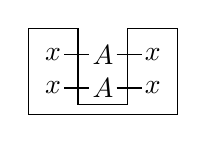
\begin{tikzpicture}[baseline=.5em, inner sep=1pt, x=1.8em, y=1.2em]
      \node (x0) at (0,0) {$x$};
      \node (A0) at (1,0) {$A$};
      \node (x1) at (2,0) {$x$};
      \draw (x0) -- (A0) -- (x1);
      \node (x2) at (0,1) {$x$};
      \node (A1) at (1,1) {$A$};
      \node (x3) at (2,1) {$x$};
      \draw (x2) -- (A1) -- (x3);
      \draw (-.5,-.8) -- (2.5,-.8) -- (2.5,1.8) -- (1.5,1.8) -- (1.5,-.5) -- (.5,-.5) -- (.5,1.8) -- (-.5,1.8) -- (-.5,-.8);
   \end{tikzpicture}
   -
   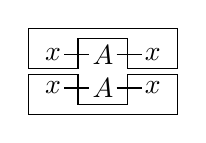
\begin{tikzpicture}[baseline=.5em, inner sep=1pt, x=1.8em, y=1.2em]
      \node (x0) at (0,0) {$x$};
      \node (A0) at (1,0) {$A$};
      \node (x1) at (2,0) {$x$};
      \draw (x0) -- (A0) -- (x1);
      \node (x2) at (0,1) {$x$};
      \node (A1) at (1,1) {$A$};
      \node (x3) at (2,1) {$x$};
      \draw (x2) -- (A1) -- (x3);
      \draw (-.5,-.8) -- (2.5,-.8) -- (2.5,.4) -- (1.5,.4) -- (1.5,-.5) -- (.5,-.5) -- (.5,.4) -- (-.5,.4) -- (-.5,-.8);
      \draw (-.5,1.8) -- (2.5,1.8) -- (2.5,.6) -- (1.5,.6) -- (1.5,1.5) -- (.5,1.5) -- (.5,.6) -- (-.5,.6) -- (-.5,1.8);
   \end{tikzpicture}
   \\&=
   \kappa_4
   \begin{tikzpicture}[baseline=(A0.base), inner sep=0pt, fill=white]
       \node (A1) at (0,0) {$A$};
       \node (bullet) at (.8,0) {$\sbullet$};
       \node[anchor=west] (A2) at (1.4,0) {$A$};
       \draw (A1.east) to[out=45,in=135] (bullet) to[out=45,in=135] (A2.west);
       \draw (A1.east) to[out=-45,in=-135] (bullet) to[out=-45,in=-135] (A2.west);
   \end{tikzpicture}
   +
   4\kappa_3\kappa_1
   \begin{tikzpicture}[baseline=(A0.base), inner sep=1pt]
       \node (A1) at (0,0) {$A$};
       \node (bullet) at (.8,0) {$\sbullet$};
       \node[anchor=west] (A2) at (1.1,0) {$A$};
       \node (bullet2) at (1.8,0) {$\sbullet$};
       \draw (A1.east) to[out=45,in=135] (bullet) -- (A2.west);
       \draw (A1.east) to[out=-45,in=-135] (bullet);
       \draw (A2.east) -- (bullet2);
   \end{tikzpicture}
   \\&\quad+
   2 \kappa_2^2 \hspace{-.5em}\trace{A,A}{2}\hspace{-.5em} + \kappa_2^2 \hspace{-1em}\trace{A}{1}\hspace{-2em}\trace{A}{1}
   \\&\quad+
   4\kappa_2\kappa_1^2
   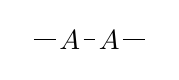
\begin{tikzpicture}[baseline=(A.base), inner sep=1pt]
       \node (bullet) at (0,0) {$\sbullet$};
       \node (A) at (.5,0) {$A$};
       \node (A2) at (1,0) {$A$};
       \node (bullet2) at (1.5,0) {$\sbullet$};
       \draw (bullet.east) -- (A.west);
       \draw (A.east) -- (A2.west);
       \draw (A2.east) -- (bullet2.west);
   \end{tikzpicture}
   +2\kappa_2\kappa_1^2
   \hspace{-1em} \trace{A}{1}\hspace{-1em}
   \vecmatvec{.5em}{\sbullet}{A}{\sbullet}
   \\&\quad+\kappa_1^4 \vecmatvec{.5em}{\sbullet}{A}{\sbullet}
   \vecmatvec{.5em}{\sbullet}{A}{\sbullet}
   \\&\quad-\big(
      \kappa_2 
      \hspace{-1em} \trace{A}{1}\hspace{-1em}
      +
      \kappa_1^2
      \vecmatvec{.5em}{\sbullet}{A}{\sbullet}
   \big)^2
   \\&=
   %%%
   2 \kappa_2^2 \hspace{-.5em}\trace{A,A}{2}\hspace{-.5em}
   +4\kappa_2\kappa_1^2
   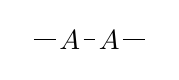
\begin{tikzpicture}[baseline=(A.base), inner sep=1pt]
       \node (bullet) at (0,0) {$\sbullet$};
       \node (A) at (.5,0) {$A$};
       \node (A2) at (1,0) {$A$};
       \node (bullet2) at (1.5,0) {$\sbullet$};
       \draw (bullet.east) -- (A.west);
       \draw (A.east) -- (A2.west);
       \draw (A2.east) -- (bullet2.west);
   \end{tikzpicture}
   \\&\quad+
   4\kappa_3\kappa_1
   \begin{tikzpicture}[baseline=(A0.base), inner sep=1pt]
       \node (A1) at (0,0) {$A$};
       \node (bullet) at (.8,0) {$\sbullet$};
       \node[anchor=west] (A2) at (1.1,0) {$A$};
       \node (bullet2) at (1.8,0) {$\sbullet$};
       \draw (A1.east) to[out=45,in=135] (bullet) -- (A2.west);
       \draw (A1.east) to[out=-45,in=-135] (bullet);
       \draw (A2.east) -- (bullet2);
   \end{tikzpicture}
   +\kappa_4
   \begin{tikzpicture}[baseline=(A0.base), inner sep=0pt, fill=white]
       \node (A1) at (0,0) {$A$};
       \node (bullet) at (.8,0) {$\sbullet$};
       \node[anchor=west] (A2) at (1.4,0) {$A$};
       \draw (A1.east) to[out=45,in=135] (bullet) to[out=45,in=135] (A2.west);
       \draw (A1.east) to[out=-45,in=-135] (bullet) to[out=-45,in=-135] (A2.west);
   \end{tikzpicture}
\end{walign}
The Matrix Cookbook lists this as
\[
   \mathrm{Var}[x^T A x]
   =
   2\mu_2^2\text{Tr}(A^2)
   + 4\mu_2 c^T A^2 c
   + 4\mu_3 c^T Aa
   + (\mu_4 - 3\mu_2^2)a^T a \tag{319}
\]
where $c = \mu_1$ is the mean of $x$,
and $a = \mathrm{diag}(A)$ is the diagonal of $A$,
and $\mu_4 = \kappa_4 + 3\kappa_2^2$ is the fourth central moment.


\section{Weighted Scalar Variable}
Let $y=w^T x$, and let $m=E[y]$, then
\begin{align*}
   \tag{321}
   \E[y] &= m = w^T \mu
   \\
   \tag{322}
   \E[(y\ominus m)^2] &= \vecmatvec{.5em}{w}{M_2}{w}
   \\
   \tag{323}
   \E[(y\ominus m)^3] &=
   \mathbin{\begin{tikzpicture}[baseline=(a0.base), inner sep=1pt]
      \node (a0) {$M_3$};
      \node[above=.3em of a0] (n0) {$w$};
      \node[right=.3em of a0] (n1) {$w$};
      \node[left=.3em of a0] (n3) {$w$};
      \draw (a0.north) -- (n0);
      \draw (a0.east) -- (n1);
      \draw (a0.west) -- (n3);
   \end{tikzpicture}}
   \\
   \tag{324}
   \E[(y\ominus m)^4] &=
   \mathbin{\begin{tikzpicture}[baseline=(a0.base), inner sep=1pt]
      \node (a0) {$M_4$};
      \node[above=.3em of a0] (n0) {$w$};
      \node[right=.3em of a0] (n1) {$w$};
      \node[below=.3em of a0] (n2) {$w$};
      \node[left=.3em of a0] (n3) {$w$};
      \draw (a0.north) -- (n0);
      \draw (a0.east) -- (n1);
      \draw (a0.south) -- (n2);
      \draw (a0.west) -- (n3);
   \end{tikzpicture}}
\end{align*}


For $x\sim N(0,1)$, we have the inequality:
\[
   \E[y^n]^{1/n} \leq \sqrt{2/\pi}\, \|w\|_2.
\]


\section{Gaussian Moments}

For a Gaussian vector $x \sim \mathcal{N}(m,M)$:
- All odd centered moments vanish: $M_3 = 0$, etc.
- Even moments can be computed via Isserlis' theorem.

For instance:
\[
\mathbb{E}[(x \ominus m)^{\otimes 4}]
=
M \otimes M + M \otimes M + \dots
\]
(summing over the different pairings of indices).

\subsection{Gaussian Integration by Parts}
If $X$ is a tensor with Gaussian entries, zero mean, and some covariance,
% General principle for Gaussian expectations.
Stein's lemma gives the following very general equation, for any differentiable function $f$:
\[
   \vcenter{\hbox{
      \import{figures/}{steins.pdf_tex}
   }}
\]
Combined with the tensor chain rule from chapter~\ref{chapter:functions}, this can be a very powerful way to evaluate many hard expectations.



\begin{align*}
E(xx^T) &= \Sigma + mm^T \tag{377} \\
E[x^TAx] &= \text{Tr}(A\Sigma) + m^TAm \tag{378} \\
\text{Var}(x^TAx) &= \text{Tr}[A\Sigma(A + A^T)\Sigma] + \cdots \tag{379} \\
&\quad +m^T(A + A^T)\Sigma(A + A^T)m \\
E[(x - m')^TA(x - m')] &= (m - m')^TA(m - m') + \text{Tr}(A\Sigma) \tag{380}
\end{align*}

If $\Sigma = \sigma^2I$ and $A$ is symmetric, then

\begin{align*}
\text{Var}(x^TAx) = 2\sigma^4\text{Tr}(A^2) + 4\sigma^2m^TA^2m \tag{381}
\end{align*}

Assume $x \sim \mathcal{N}(0, \sigma^2I)$ and $A$ and $B$ to be symmetric, then

\begin{align*}
\text{Cov}(x^TAx, x^TBx) = 2\sigma^4\text{Tr}(AB) \tag{382}
\end{align*}

\subsection{Cubic forms}

Assume $x$ to be a stochastic vector with independent coordinates, mean $m$ and covariance $M$

\begin{align*}
E[xb^Txx^T] &= mb^T(M + mm^T) + (M + mm^T)bm^T \tag{383} \\
&\quad +b^Tm(M - mm^T)
\end{align*}

\subsection{Mean of Quartic Forms}

\begin{align*}
E[xx^Txx^T] &= 2(\Sigma + mm^T)^2 + m^Tm(\Sigma - mm^T) \\
&\quad +\text{Tr}(\Sigma)(\Sigma + mm^T) \\[1em]
E[xx^TAxx^T] &= (\Sigma + mm^T)(A + A^T)(\Sigma + mm^T) \\
&\quad +m^TAm(\Sigma - mm^T) + \text{Tr}[A\Sigma](\Sigma + mm^T) \\[1em]
E[x^Txx^Tx] &= 2\text{Tr}(\Sigma^2) + 4m^T\Sigma m + (\text{Tr}(\Sigma) + m^Tm)^2 \\[1em]
E[x^TAxx^TBx] &= \text{Tr}[A\Sigma(B + B^T)\Sigma] + m^T(A + A^T)\Sigma(B + B^T)m \\
&\quad +(\text{Tr}(A\Sigma) + m^TAm)(\text{Tr}(B\Sigma) + m^TBm)
\end{align*}

\begin{align*}
E[a^Txb^Txc^Txd^Tx] &= (a^T(\Sigma + mm^T)b)(c^T(\Sigma + mm^T)d) \\
&\quad +(a^T(\Sigma + mm^T)c)(b^T(\Sigma + mm^T)d) \\
&\quad +(a^T(\Sigma + mm^T)d)(b^T(\Sigma + mm^T)c) - 2a^Tmb^Tmc^Tmd^Tm
\end{align*}

\begin{align*}
&E[(Ax + a)(Bx + b)^T(Cx + c)(Dx + d)^T] \\
&= [A\Sigma B^T + (Am + a)(Bm + b)^T][C\Sigma D^T + (Cm + c)(Dm + d)^T] \\
&\quad +[A\Sigma C^T + (Am + a)(Cm + c)^T][B\Sigma D^T + (Bm + b)(Dm + d)^T] \\
&\quad +(Bm + b)^T(Cm + c)[A\Sigma D^T - (Am + a)(Dm + d)^T] \\
&\quad +\text{Tr}(B\Sigma C^T)[A\Sigma D^T + (Am + a)(Dm + d)^T]
\end{align*}

\begin{align*}
&E[(Ax + a)^T(Bx + b)(Cx + c)^T(Dx + d)] \\
&= \text{Tr}[A\Sigma(C^TD + D^TC)\Sigma B^T] \\
&\quad +[(Am + a)^TB + (Bm + b)^TA]\Sigma[C^T(Dm + d) + D^T(Cm + c)] \\
&\quad +[\text{Tr}(A\Sigma B^T) + (Am + a)^T(Bm + b)][\text{Tr}(C\Sigma D^T) + (Cm + c)^T(Dm + d)]
\end{align*}

See [7].


\subsection{Mixture of Gaussians}
For a mixture of Gaussians:
\[
   x \sim \sum_k \pi_k \mathcal{N}(m_k, M_k),
\]
the moments are weighted sums:
\[
   E[x] = \sum_k \pi_k m_k, \quad
   \mathrm{Var}[x] = \sum_k \pi_k (M_k + m_k m_k^T) - \left(\sum_k \pi_k m_k\right)\left(\sum_k \pi_k m_k\right)^T.
\]
Higher moments similarly combine via linearity.


\begin{align*}
E[x] &= \sum_k \rho_k m_k \tag{384} \\[1em]
\text{Cov}(x) &= \sum_k\sum_{k'} \rho_k\rho_{k'} (\Sigma_k + m_km_k^T - m_km_{k'}^T) \tag{385}
\end{align*}

\subsection{Derivatives}
Derivatives of moments with respect to $m$ or $M$ can be found by differentiating under the integral sign, and using Stein's lemma for Gaussian cases.

\section{Exercises}
\begin{exercise}
   \begin{align*}
   \mathbb{E}[(A\mathbf{x} + a)(A\mathbf{x} + a)^T (A\mathbf{x} + a)] = 
   \text{Adiag}(A^T A) v_3 \\
   + [2 AMA^T + (A\mathbf{x} + a)(A\mathbf{x} + a)^T] (Am + a) \\
   + \text{Tr}(AMA^T)(Am + a)
   \end{align*}

   \begin{align*}
   \mathbb{E}[(A\mathbf{x} + a) b^T (C\mathbf{x} + c)(D\mathbf{x} + d)^T] = 
   (A\mathbf{x} + a) b^T (CMD^T + (Cm + c)(Dm + d)^T) \\
   + (AMC^T + (Am + a)(Cm + c)^T) b(Dm + d)^T \\
   + b^T (Cm + c)(AMD^T - (Am + a)(Dm + d)^T)
   \end{align*}
\end{exercise}
\begin{exercise}
   Find more identities in the \href{http://www.ee.ic.ac.uk/hp/staff/dmb/matrix/expect.html}{Matrix Reference Manual} and try to prove them.
   Also try to verify your derivations using tensorgrad.
\end{exercise}
